% REPORT.TEX - University of Warwick Reports / Dissertations / Projects
% 
% Author - Chris Quinn 28/06/2020
% 
%
% A template for students and masters dissertations, flexible for your
% needs.
%
% This is the main .tex which will tell the compiler to include everything, 
% each chapter/section is then in folders for convenience, as you include more 
% images it can get harder and harder to manage.
%
% First things first, declaration of the document class along with the packages % we need.
%
% P.S. Sorry about the back to the future references, I used them to show some 
% example work possible




\documentclass[pdftex,10pt,a4paper,oneside]{article}
%Can change the pt, papersize etc.

\usepackage{amsmath} %For both in-line and equation mode
\numberwithin{equation}{section} %Numbering of our equations per section
\usepackage{algorithm}
\usepackage{algorithmic} %Algorithm styles, need to be nested for the example shown
\usepackage{fancyhdr} %For our headers
\usepackage{graphicx} %Inserting images
\usepackage{lipsum}  %Blank text fill, delete me when finished
\usepackage{setspace} %Spacing on the front page for crest and titles
\usepackage[]{fncychap} % Styles can be Sonny, Lenny, Glenn, Conny, Rejne, Bjarne and Bjornstrup
\usepackage[hyphens]{url} %Deals with hyphens in urls to make them clickable
\usepackage{xcolor} %Great if you want coloured text
\usepackage{tabularx}
\usepackage[toc,page]{appendix} %Take a wild guess slick
\usepackage{hhline}
\usepackage[most]{tcolorbox}
\usepackage{lineno}
\usepackage{amsmath,amssymb,amsfonts, amsthm, mathabx}
\usepackage{float}
\usepackage{enumitem}
\usepackage{placeins}
\usepackage{algorithmic}
\usepackage{xltabular}
\usepackage{graphicx}
\usepackage{lipsum}
\usepackage{textcomp}
\usepackage{xcolor}
\usepackage{tikz}
\usepackage[inner=2.5cm,outer=1.5cm,bottom=2cm]{geometry}
\usepackage[symbols]{glossaries}
\usepackage{subcaption}


% \newtheorem{theorem}{Theorem}[section]
% \newtheorem{conjecture}[theorem]{Conjecture}
% \newtheorem{proposition}[theorem]{Proposition}
% \newtheorem{lemma}[theorem]{Lemma}
% \newtheorem{claim}[theorem]{Claim}
% \newtheorem{corollary}{Corollary}[theorem]
% \newtheorem{definition}{Definition}[section]



\makeglossaries
\loadglsentries[\symboltype]{Preamble/Notation}
\usepackage{Tex-Definitions/tex-commands}
\usepackage{Tex-Definitions/tex-definitions}



%KEEP THIS ONE LAST it's quite buggy, it allows you to click on links within the pdf and web links without changing the colour. The mouse cursor simply changes its icon to indicate to the user. Great tool - still awkward
\usepackage[hidelinks]{hyperref}



%This will tell the compiler to do the header style, page and spacing between the header and text
\fancyhf{}
\pagestyle{fancy}
\renewcommand{\headrulewidth}{0.2pt}


%%%%%%%%%%%%%%%%%%%%%%%%%% DOCUMENT STARTS %%%%%%%%%%%%%%%%%%%%%%%%%%%%%



%Lets begin the document, some chapters have examples in to give you an idea 
\begin{document}


\glsaddall

% !TEX root =  ../Report.tex

\thispagestyle{empty}

\begin{spacing}{2}
	\begin{center}
		
\includegraphics[scale = 0.45]{Preamble/WarwickCrest.pdf}
		%Two images here for University of Warwick students, the colour crest and the black and white crest. Replace as appropriate!
	\end{center}
	\vspace{5mm}
	\begin{center}
		\textbf{\begin{LARGE}
		Counting Complexity of PureCircuit -1
		\end{LARGE}}
		\vspace{5mm}
	\end{center}
	\begin{center}
		{\large CS907 Dissertation Project}\\
		\vspace{20mm}
	\end{center}
	\begin{center}
		\textbf{\large Christos Demetriou 2018918}
		\vspace{20mm}
	\end{center}
	\begin{center}
	     {\large Supervisor: Dr. Christian Ikenmeyer }\\
		\textbf{\large Department of Computer Science}\\
		{\large University of Warwick}\\
		{\large 2024-2025\\}
	\end{center}
\end{spacing}

\pagenumbering{roman}



\section*{Abstract}
\addcontentsline{toc}{section}{Abstract}
\vspace{2cm}

\large
When this thing gets up to 88 mph, you're gonna see some serious s$\cdot \cdot \cdot$.\\

\vspace{1cm}

\noindent \textit{Keywords: Flux Capacitor, 1.21 Gigawatts, Calvin Klein}
\section*{Acknowledgements}
\addcontentsline{toc}{section}{Acknowledgements}

\vspace{2cm}

\large

Always good to acknowledge people. %(yes, there are definitely people to acknowledge )
%Comment the whole thing out if you don't want it

\section*{Abbreviations}
\addcontentsline{toc}{section}{Abbreviations}
\large 
Pure Circuit \hfill PC\\





\tableofcontents

% Once you start inserting figures, tables and algorithms then they % will start appearing here in the lists. 
%
% The captions and names you give them will appear here. The 
% numbering can either be:
%
%     Natural (1,2,3,...) 
%     Sectional (1.1, 1.2 for chapter 1. 2.1, 2.2,... for chapter 2) 



\listoffigures
\addcontentsline{toc}{section}{List of Figures}
\numberwithin{figure}{section}

\listoftables
\addcontentsline{toc}{section}{List of Tables}
\numberwithin{table}{section}

%Delete me if you're not putting algorithms in or you don't want it as contents. Same applies with the two above ^
\listofalgorithms
\addcontentsline{toc}{section}{List of Algorithms}
\numberwithin{algorithm}{section}

\newpage


\MakeLinkTarget*{symbol}%
\addcontentsline{toc}{section}{List of Symbols}\printglossary[type=symbols, title={List of Symbols}, style=list,nonumberlist]
\clearpage


\pagenumbering{arabic}

\lfoot{\centering \thepage}

% !TEX root =  ../Report.tex

\section{Introduction}
\label{sec:Introduction} 

% !TEX root =  ../Report.tex
\section{Theoretical Preliminaries}

Our work lies in the intersection of the three core fields:
counting complexity, total search problems and Kleene logic.

\subsection{Search problems}
We offer brief preliminaries to function problems and the different kinds that exist.
First and foremost when

\begin{definitionbox}{Search Problems}{search-problems}
    \textbf{Search problems} can be defined as relations $R \subseteq \mathbb{B}^* \times \mathbb{B}^*$,
    where given $x \in \mathbb{B}^*$, we want to find $y \in \mathbb{B}^*$  such that $xRy$.

    \textbf{Total Search problems} are search problems such that for each input, there must exist at least one solution.
\end{definitionbox}

Like decision problems, we can define their search analogues
using the definitions in \ref{def:fnp-tfnp}.
Moreover, we use the \textit{Levin reductions} \ref{def:levin-reductions} to associate
two problems.


\begin{definitionbox}{$\scn{FNP}$ and $\scn{TFNP}$}{fnp-tfnp}
    \label{def:fnp-tfnp}
    \textbf{FNP} are \textit{search problems} such that there exists poly-time TM $M: \mathbb{B}^* \to \mathbb{B}$
    and a poly function $p : \mathbb{N} \to \mathbb{N}$ such that:
    $$
        \forall x \in \mathbb{B}^*, y \in \mathbb{B}^{p(|x|)}: xRy \iff M(x,y) = 1
    $$
    Lastly $\textbf{TFNP} = \{L \in \textbf{FNP} \mid L \text{ is total}\}$
\end{definitionbox}

\begin{definitionbox}{Levin Reductions}{levin-reductions}
    \label{def:levin-reductions}
    Given two search problems $R,R'$,
    a pair of poly-time computable functions \(f,g\) where \(f,g: \{0,1\}^* \to \{0,1\}^*\), is
    called a \textit{Levin reduction}, if
    \begin{gather*}
        S_R \triangleq \{x \mid \exists y : xRy\} \\
        R(x) \triangleq \{y \in \{0,1\}^* \mid xRy\} \\
        \forall x \in \{0,1\}^*: x \in  S_R \implies f(x) \in S_{R'}\\
        \forall x \in S_R, y' \in R'(f(x)): (x,g(x,y)) \in R
    \end{gather*}
\end{definitionbox}

Within the current project, we are mainly interested with the total search problems or at least a specific hierarchy,
as shown in figure \ref{..}. These problems were introduced by various researchers as seen in {},
and all such classes the guarantee of an existence of a solution by using
some combinatorial property of the nature of the problem but can be very difficult to find. In the current project we are mainly interested
in \texttt{PPAD}, known as ``Polynomial Parity of Augmented DiGraphs'', created by Papadimitriou \cite{papadimitriou_ComplexityParityArgument_1994}.
We will give a formal definition of the class as well as several cornerstone problems that we will refer to in the upcoming chapters.

We will first introduce the \textit{EndOfLine} problem \ref{def:eol-ppad}by Papadimtirou \cite{papadimitriou_ComplexityParityArgument_1994},
which takes advantage of the combinatorial fact of directed graphs where a pair of odd-degree vertices come in pairs.

\begin{definitionbox}{\textit{EndOfLine} problem \cite{papadimitriou_ComplexityParityArgument_1994}}{eol-ppad}\
    \label{def:eol-ppad}
    Given poly-sized circuits $S, P \in \mathbb{B}^n \to \mathbb{B}^n$,
    we define a digraph $G = (V,E)$, such that $V= \mathbb{B}^n$ and $E$ defined as:
    $$
        E = \{(x,y) \in V^2: S(x) = y \wedge P(y) = x\}
    $$
    We define source nodes as $v \in V: \textit{deg}(v) = (0,1)$  and sink nodes as
    $\textit{deg}(v) = (1,0)$.
    We also syntactically ensure that the $0^n$ node is always a source, meaning
    $S(P(0^n)) \neq 0 \wedge P(S(0^n)) = 0^n$.
    A node $v \in V$ is a solution \textit{iff} $\textit{in-deg}(v) \neq \textit{out-deg}(v)$.
\end{definitionbox}

\begin{figure}
    \centering
    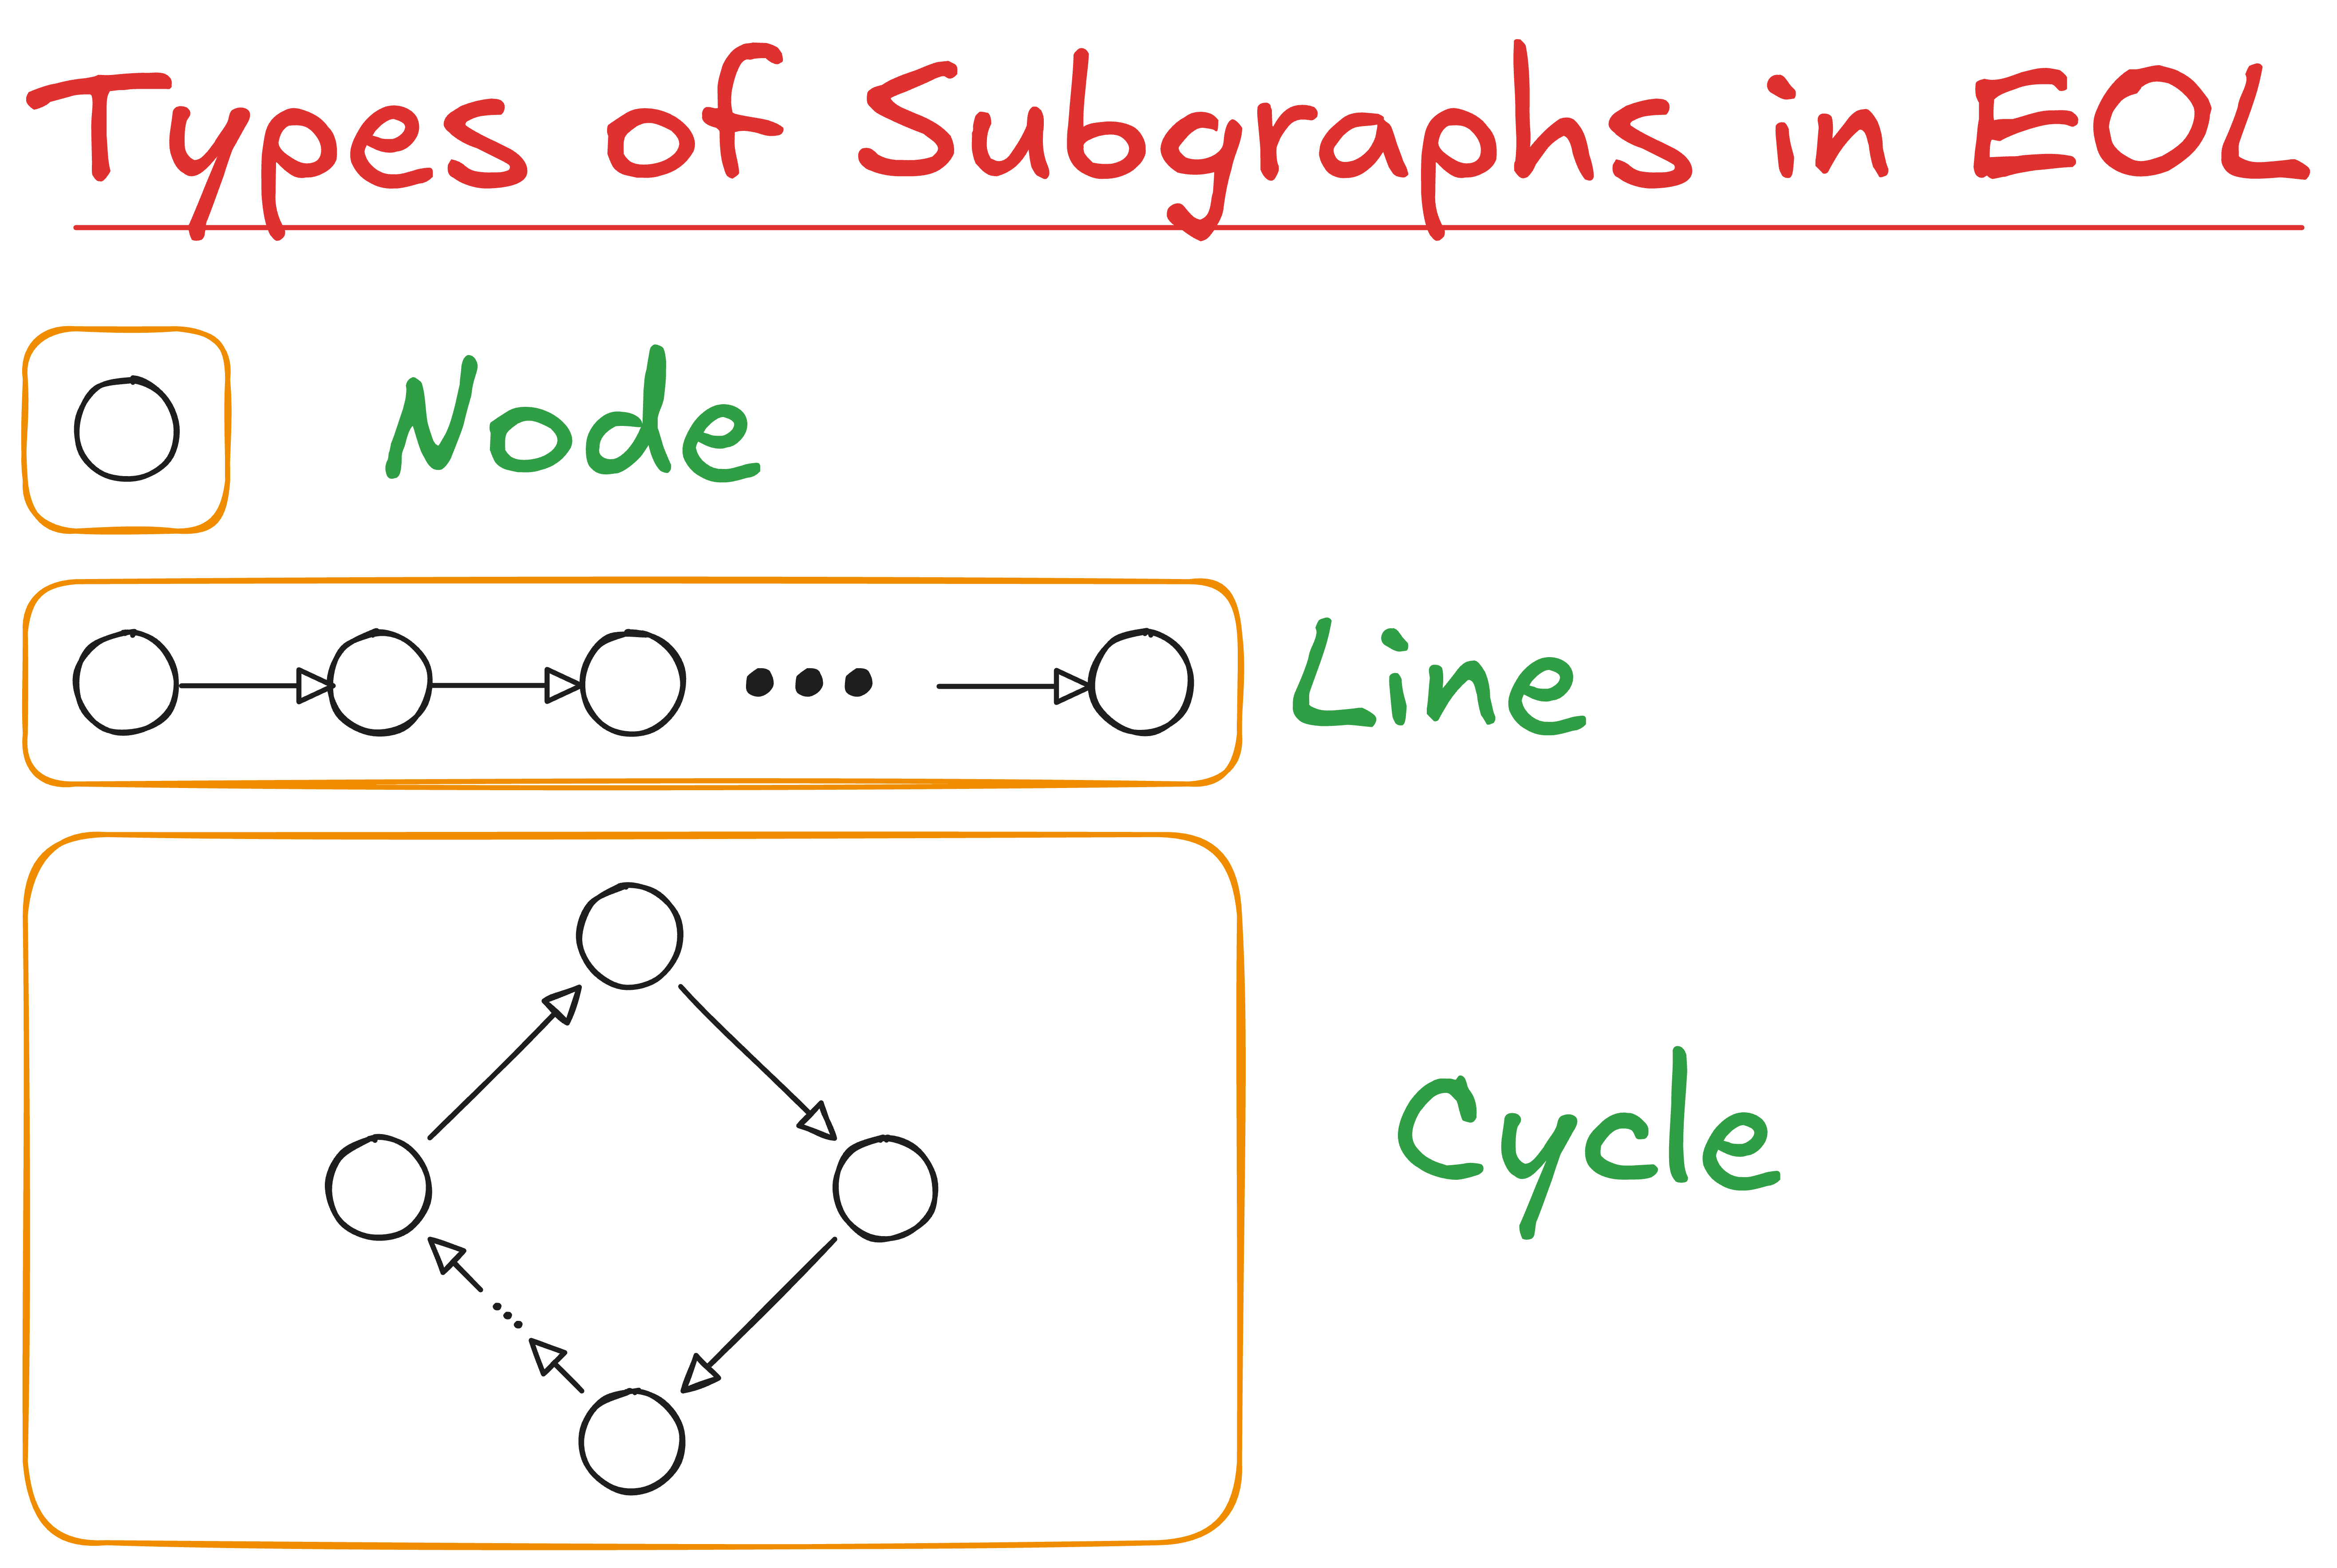
\includegraphics[width=0.7\linewidth]{assets/eol-subgraphs.png}
    \caption{Types of subgraphs in \textsc{EndOfLine}}
    \label{fig:eol-subgraphs}
\end{figure}

\vspace{0.2cm}

An illustrative example of an \textsc{EndOfLine} instance can be seen in figure \ref{fig:eol-subgraphs}.
From this problem, we define the \textsc{PPAD} complexity class \ref{def:ppad-complexity-class}.

\begin{definitionbox}{\scn{PPAD} complexity class \cite{papadimitriou_ComplexityParityArgument_1994}}{ppad-complexity-class}
    \textsc{PPAD} is defined as the set of search problems that
    are \textit{levin reducible} \ref{def:levin-reductions} to the \scn{EndOfLine} problem \ref{def:eol-ppad}.
\end{definitionbox}

\subsubsection{EndOfLine variants and extensions}
%% TODO: ADD MISSING REFERENCES and CLEANUP
We want introduce a small number of the several key variants of the \textit{EndOfLine} that have been created in the past.
Alexandros et al. in the paper {} was able to demonstrate that for several modifications of the original problem such as adding
$k$ known sources, where $k$ can be a polynomial function with respect to the number of sources. Moreover, people
have experimented with changing the degrees of the graphs, as demonstrated by Ikenmeyer et al. \cite{ikenmeyer_WhatWhatNot_2022},
with the problems such as $\textsc{SourceOrExcess}(k,1)$ where $k$ it the maximum in-degree for each node.
All these problems remain \textbf{PPAD} complete. More interestingly, Papadimitriou et al. {} and
Alexandros et al. {} were able to demonstrate that in the more general case of superpolynomial graphs,
if we bound the in-degree and out-degree of each node to some polynomial of the input size, then problem remains \textbf{PPAD}.
We will give the main definitions to the most relevant problems in the upcoming sections.

\begin{definitionbox}{\scn{SourceOrExcess} problem \cite{ikenmeyer_WhatWhatNot_2022}}{source-or-excess}
    We define as $\textit{SourceOrExcess}(k,1)$ for $k \in \mathbb{N}_{\geq 2}$
    the search problem as such: Given a poly-sized successor circuit $S : \mathbb{B}^n$
    and a set of predecessor poly-sized circuits $\{P_i\}_{i \in [k]}$, we define
    the graph $G = (V,E)$ such that, $V = \mathbb{B}^n$ and $E$ as:
    $$
        \forall x, y \in V: (x,y) \in E \iff (S(x) = y) \wedge \bigvee_{i \in [k]} P_i(y) = x
    $$
    We ensure that $0^n$ is as source, meaning $\text{deg}(0^n) = (0,1)$.
    A valid solution is a vertex $v$ such that $\textit{in-deg}(v) \neq \textit{out-deg}(v)$.
\end{definitionbox}


%% TODO REFERENCE
In addition to the aforementioned adjustments, researchers were able to give a topological interpretation
to the \scn{EndOfLine} \ref{def:eol-ppad} problem, by creating embeddings of the graph
into 2D or 3D spaces as demonstrated by several researchers {deligkas, chen, Alexandros}.
We will mainly look at two of these problems, known as \textsc{RLeafD} and \textsc{2D-EOL}
created by Chen et al. and Alexandros respectevily.

%% TODO REFERENCE
\begin{definitionbox}{\scn{2D-EOL} problem {}}{2d-eol}
    \label{2d-eol}
    \textbf{Input}: Two poly-sized circuits $P,S: \{0,1\}^{2n} \to \{0,1\}^{2n}$ where $P(0^{n}, 0^{n}) = (0^{n},0^{n}) \neq S(0^{n}, 0^{n})$.
    \textbf{Output}: A point $x \in \{0,1\}^{2n}$ such that one of the following conditions are satisfied:
    \begin{enumerate}
        \item Sinks: $P(S(x)) \neq x$
        \item Sources: $S(P(x)) \neq  x \wedge x \neq 0^n$
        \item Invalid successor: $x - S(x) \not\in \{(0,0), (0,1), (0,-1), (1,0), (-1,0)\}$
        \item Invalid predecessor: $x - P(x) \not\in \{(0,0), (0,1), (0,-1), (1,0), (-1,0)\}$
    \end{enumerate}
\end{definitionbox}

The above description defines a superpolynomial such that an edge $(x,y) \in E$
if and only if $S(x) = y \wedge P(y) = x$ as well as the closeness constraint $\|x-S(x)\|_1 \leq 1$.
We will now refer to a special case of  \scn{2D-EOL} known as \scn{RLeafD} by Chen et al. where
they give a planar embedding of any graph $G$ onto a 2D plane. We find this construction useful for our results
and therefore will investigate this method further.

\paragraph{Planar Graph Embedding}
We define the graph embedding of a graph $G = (V,E)$ as $G_n = (V_n, E_n)$ where $|V| = n$ and $V_n$ is defined as
\[
    \forall n \in \mathbb{N}:  V_n \triangleq \Big\{\mathbf{u} \in \mathbb{N}_0^2\mid \mathbf{u}_1 \leq 3(n^2 - 1) , \mathbf{u}_2 \leq 6(n - 1) + 3 \Big\}
\]
$G$ can have any in- and out-degree.
For a vertex $i \in V$, we correspond it to the node $(0, 6i)$ in the embedded version.
To define the edge set, we will first introduce the following notations.

\begin{definitionbox}{$E(\mathbf{p}^1,\mathbf{p}^2 )$}{rleaf-edge}
    \label{def:rleaf-edge}
    Given two points $\mathbf{p}^1, \mathbf{p}^2 \in V_n$ we define the set of edges
    $E(\mathbf{p}^1, \mathbf{p}^2)$ as:
    $$
        E(\mathbf{p}^1, \mathbf{p}^2) \triangleq \begin{cases}
            \{(\alpha, k) \mid k \in \mathbb{N} : \min\{\mathbf{p}^1_2, \mathbf{p}^2_2\} \leq k  \leq \max\{\mathbf{p}^1_2, \mathbf{p}^2_2\}\} & \text{if }\mathbf{p}^1_1 = \mathbf{p}^2_1 = \alpha \\
            \{(k, \alpha) \mid k \in \mathbb{N} : \min\{\mathbf{p}^1_1, \mathbf{p}^2_1\} \leq k  \leq \max\{\mathbf{p}^1_1, \mathbf{p}^2_1\}\} & \text{if }\mathbf{p}^1_2 = \mathbf{p}^2_2 = \alpha \\
            \emptyset                                                                                                                          & \text{otherwise}                                   \\
        \end{cases}
    $$
\end{definitionbox}

\begin{definitionbox}{$E_{ij}$}{rleaf-full-edge}
    \label{def:rleaf-full-edge}
    Given an edge of the original graph $(i,j) \in E$, we define the set of edges $E_{ij}$ as:
    \begin{align*}
        \mathbf{p}^1 & = (0, 6i)                                                                           \\
        \mathbf{p}^2 & = (3(ni + j), 6i)                                                                   \\
        \mathbf{p}^3 & = (3(ni + j), 6j + 3)                                                               \\
        \mathbf{p}^4 & = (0, 6j + 3)                                                                       \\
        \mathbf{p}^4 & = (0, 6j)                                                                           \\
        E_{ij}       & \triangleq E(\mathbf{p}^1\mathbf{p}^2) \cup \dots  \cup E(\mathbf{p}^4\mathbf{p}^5)
    \end{align*}
\end{definitionbox}

To formally define $E_n$, we first split $E_n$ into two disjoint sets $E^1_n$ and $E^2_n$.
We define $E^1_n$ as  $\bigcup_{ij \in E} E_ij$. The graph generated by
$(V_n, E_n)$ has some special properties such as, $\forall v \in V_n: \text{in-deg}(v) + \text{out-deg}(v) \leq 4$
and $\forall v \in V_n: \text{deg}(v) = 4 \implies \text{in-deg}(v) =2 = \text{out-deg}(v)$. For every
4-degree vertex, we add $4$ additional edges as depicted in the figure \ref{fig:chap-2:rleafd-new-edges}
depicted in blue and add them to $E^2_n$.

\begin{figure}[h!]
    \centering
    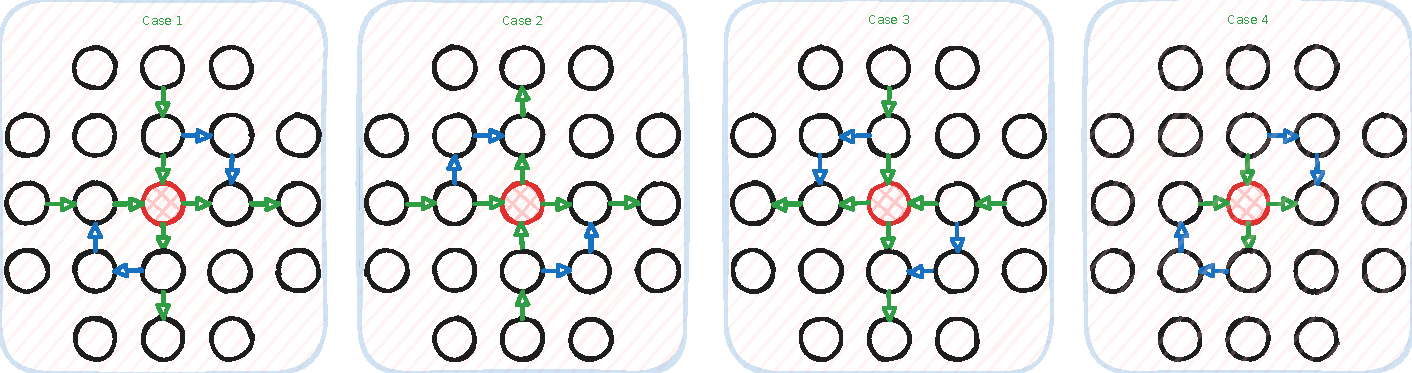
\includegraphics[width=\textwidth]{Chapter2/rleafd.pdf}
    \caption{Figure redrawn from \cite{chen_Complexity2DDiscrete_2009}}
    \label{fig:chap-2:rleafd-new-edges}
\end{figure}


Given the above we have a full description of $G_n$. A visual explanation
can be seen in figure \ref{fig:chap-2:edge-rleaf} and an example of the $K_3$ complete graph in
figure \ref{fig:chap-2:rleaf-k3}

\begin{figure}[h!]
    \centering
    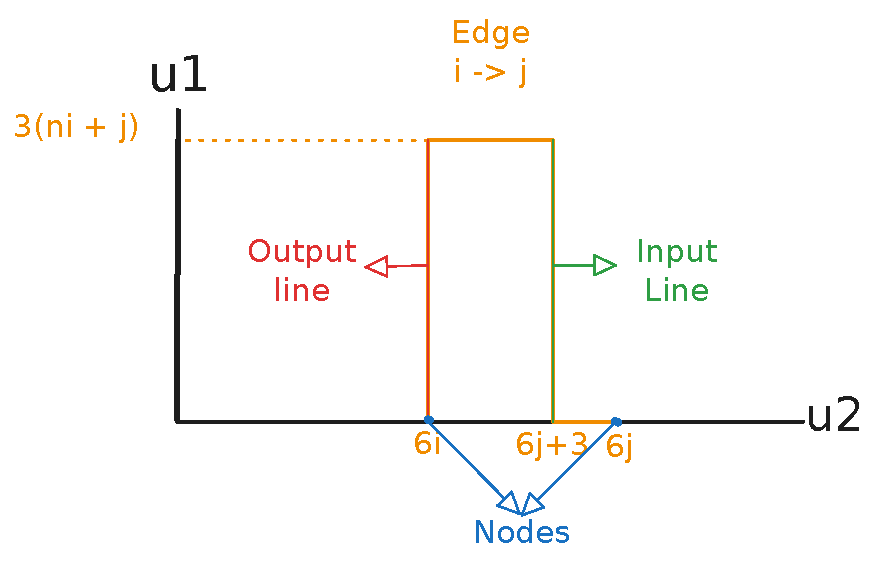
\includegraphics[width=0.5\textwidth]{Chapter2/rleaf-edge-example.pdf}
    \caption{Edge between points $i,j$ of the original graph. Main observation is the fact that each point comes with a pair of
        exponentially long lines, which we refer to as the input output lines.}
    \label{fig:chap-2:edge-rleaf}
\end{figure}

\begin{figure}[h!]
    \centering
    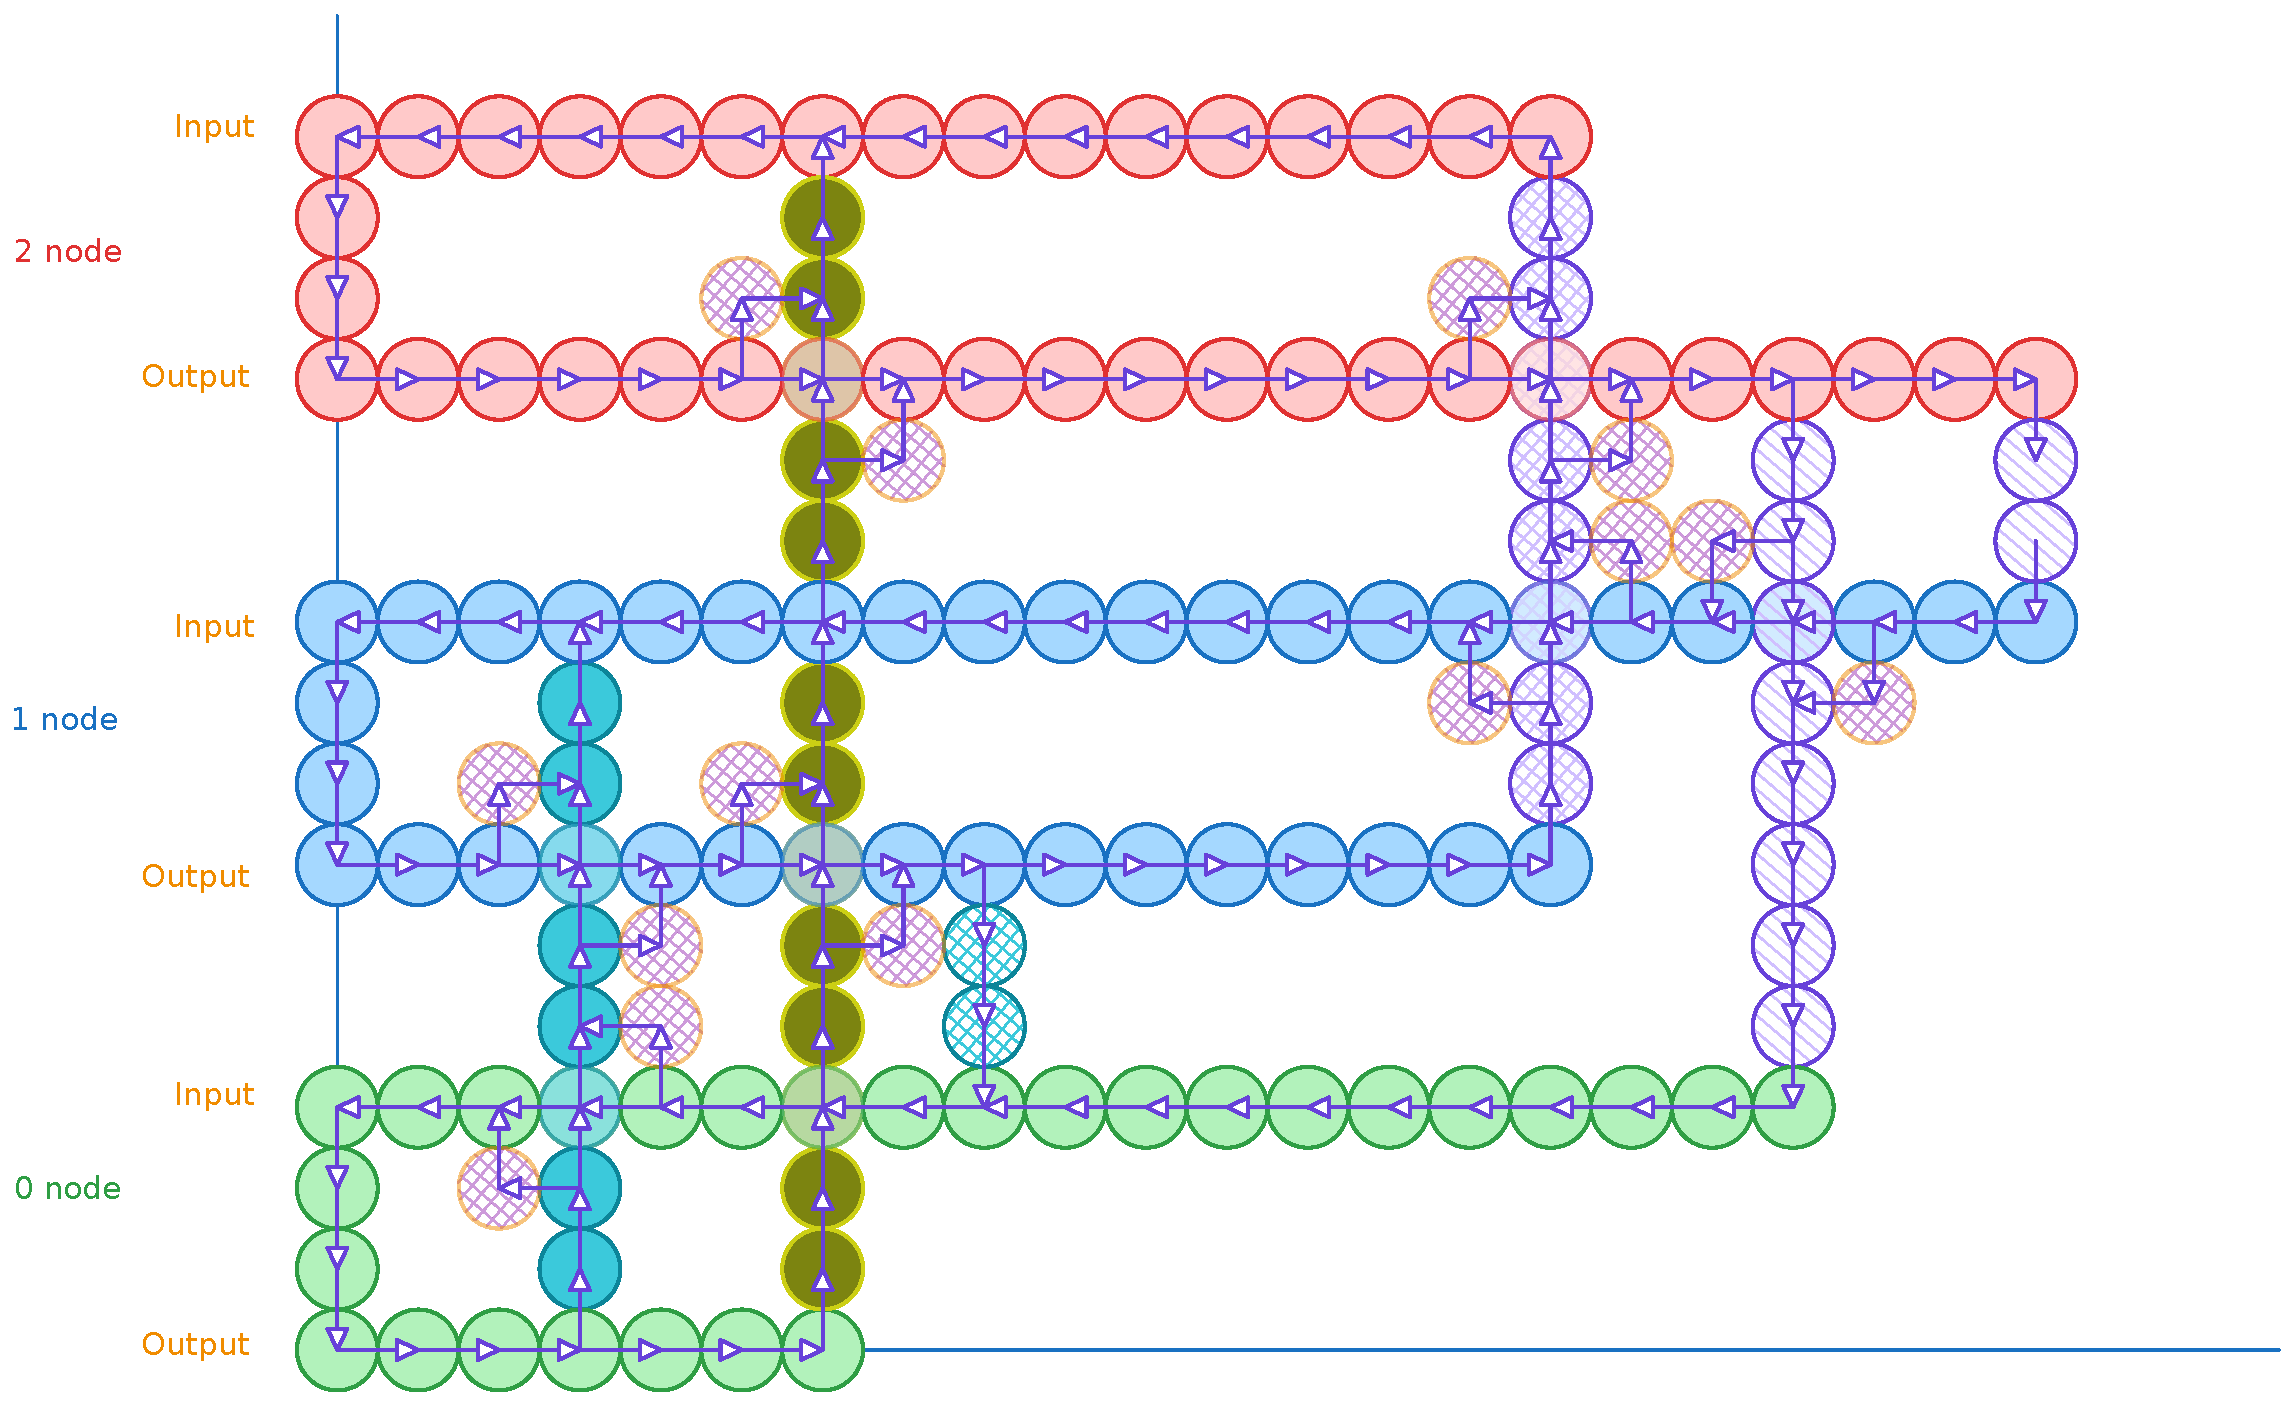
\includegraphics[width=0.7\textwidth]{Chapter2/rleaf-k3-example.pdf}
    \caption{$K_3$ graph construction. Combinations of colours indicate an edge between the two nodes. Solid dots indicate edges from $0$,
        crossed lines indicate edges from $1$ and stripped lines indicate edges from $2$. We Add two coloured stripped circles on the
        4 degree nodes to indicate the $E^2_n$ edges.}
    \label{fig:chap-2:rleaf-k3}
\end{figure}


\paragraph{\scn{RLeafD} problem}
We denote $C_n$ as the set of planar graphs $G_n = (V_n,E_n)$ such that
$\forall \mathbf{u} \in V_n: \textit{in-deg}(v) \leq 1 \wedge \textit{out-deg}(v) \leq 1$. From that we define
the class of problems \textsc{RLeafD} as in definition \ref{def:rleafd-problem}.


\begin{definitionbox}{RLeafD problem \cite{chen_Complexity2DDiscrete_2009}}{rleafd-problem}
    \label{def:rleafd-problem}
    \textbf{Input}: A tuple $(K, 0^k)$ such that $k \in \mathbb{N}$ and $K$ is a poly-time TM
    which describes a graph in $G \in C_n$.
    More specifically, $K$ is a function $V_{2^k} \to V_{2^k} \cup \{\bot\}$ such that
    $$
        (a,b) \in E_n \iff K(a) = (\cdot, b) \wedge  K(b) = (a, \cdot)
    $$
    \textbf{Output}: $v \in V_{2^k} \setminus \{0^n\}$ such that
    $\exists a \in V_{2^k}: K(v) = (\cdot, a) \vee K(v) = (a, \cdot)$
\end{definitionbox}

\paragraph{Embedding \scn{EndtofLine}}
Chen et al. \cite{chen_Complexity2DDiscrete_2009} demonstrated how every \scn{EndOfLine} can be reduced to a
\textsc{RLeafD} problem. Key insight, is the observation that every planar embedding of a graph of an \scn{EndOfLine}
has the following property:
$$
    \forall v \in V_n: \textit{deg}(v) \in \{(0,0), (1,1), (1,0), (0,1), (2,2)\}
$$
Using as reference the figure \ref{fig:chap-2:edge-rleaf}, we remove all the edges of nodes with degree of $(2,2)$.
This in a way creates a different graph but the key insight is that the number of sources or sinks remain the same as we are essentially redirecting the lines
as we can see from the figure \ref{fig:chap-2:rleaf-eol}. We will use these reductions in later sections to demonstrate reductions with excess problems as well.

\begin{figure}[h!]
    \centering
    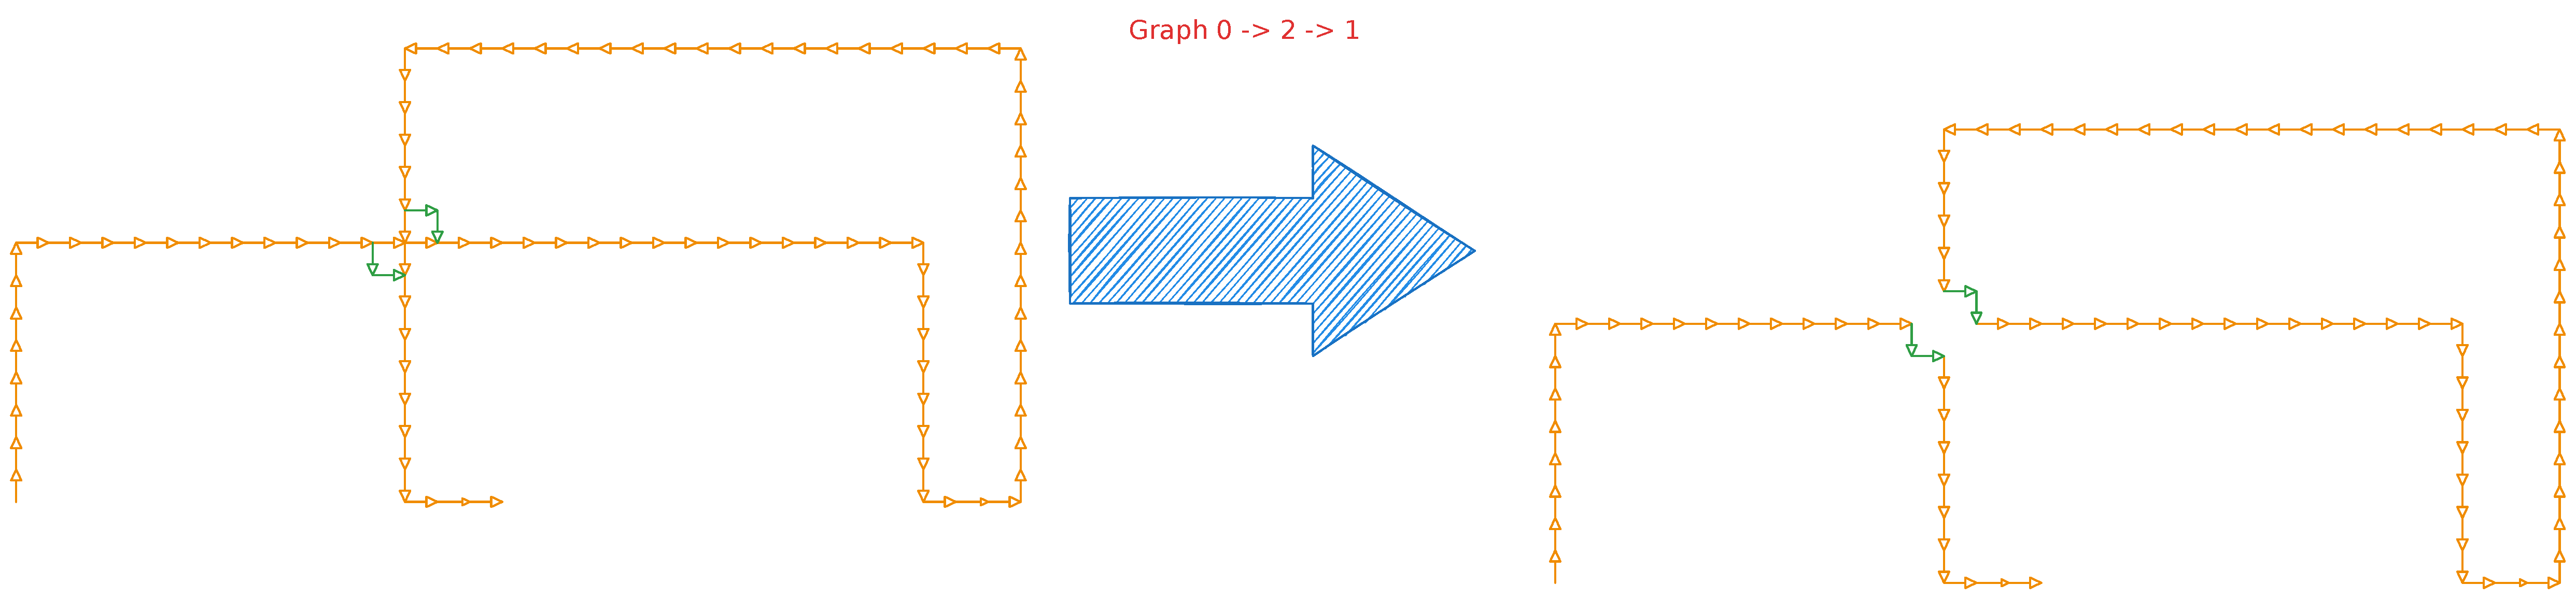
\includegraphics[width=0.7\textwidth]{Chapter2/reduced-EOL.pdf}
    \caption{Depiction of the edge removal. Main idea is that this we keep the number of sources or sinks as well as invertible (we can trace the source or sink from the original instance),
        despite losing a lot of graph information.}
    \label{fig:chap-2:rleaf-eol}
\end{figure}




\paragraph{The PureCircuit problem}
\label{par:pure-circ-def}

The definition of \textsc{PureCircuit} is based Kleene's three-valued strong logic of indeterminacy,
which extends the traditional binary logic \cite{kleene_IntroductionMetamathematics_2009}.
This problem was created by Deligkas et al. \cite{deligkas_PureCircuitTightInapproximability_2024}
to demonstrate the hardness of approximating \textsc{PPAD} problems and was shown to be \textsc{PPAD-complete}.


\begin{definitionbox}{\scn{PureCiruit} Problem Definition \cite{deligkas_PureCircuitTightInapproximability_2024}}{purecircuit-def}
    An instance of \textit{PureCircuit} is given by vertex set $V= [n]$ and gate set $G$ such that
    $\forall g \in G: g=(T,u,v,w)$ where $u,v,w \in V$ and $T \in \{\text{NOR}, \text{Purify}\}$.
    Each gate is interpreted as:
    \begin{enumerate}
        \item \textit{NOR}: Takes as input $u,v$ and outputs $w$
        \item \textit{Purify}: Takes as input $u$ and outputs $v,w$
    \end{enumerate}
    And each vertex is ensured to have $\text{in-deg}(v) \leq 1$.
    A solution to input instance $(V,G)$ is denoted as an assignment $\mathbf{x} : V \to \{0, \bot, 1\}$
    such that for all gates $g = (T,u,v,w)$ we have:
    \begin{enumerate}
        \item \textit{NOR}:
              \begin{gather*}
                  \mathbf{x}[u] = \mathbf{x}[v] = 0 \implies \mathbf{x}[w] = 1\\
                  (\mathbf{x}[u] =1 \vee \mathbf{x}[v] =1) \implies \mathbf{x}[w] = 0 \\
                  \text{otherwise} \implies \bot
              \end{gather*}

        \item \textit{Purify}:
              \begin{gather*}
                  \forall b \in \mathbb{B}: \mathbf{x}[u] = b \implies \mathbf{x}[v] = b \wedge \mathbf{x}[w] =  b\\
                  \, \mathbf{x}[u] = \bot \implies \{\mathbf{x}[v] \cup \mathbf{x}[w] \} \cap \mathbb{B}\neq \emptyset
                  \, \, \end{gather*}
    \end{enumerate}
\end{definitionbox}

In addition to the gates above, we will make use of the standard set of gates $\{\vee, \wedge, \neg\}$,
whose behaviour is depicted in the tables \ref{tab:three-val-logic}.
Moreover, we will make use of the \textit{Copy} gate which we can define as $\textit{Copy}(x) = \neg (\neg x)$.
These gates are well defined based on the \textit{NOR} gate as shown by Deligkas et al. \cite{deligkas_PureCircuitTightInapproximability_2024}
and do not directly affect the complexity of the problem.
Furthermore, with respect to the \textit{Purify} gate,
Deligkas et al. \cite{deligkas_PureCircuitTightInapproximability_2024} showed that the only \textit{Purify} solutions essential
for \textsc{PPAD-completeness} are $\{(0,\bot), (\bot,1), (0,1)\}$, and the addition of more solutions does not affect its complexity.
We will base our constructions around that limited set of solutions.
We acknowledge that this simplified variant of the problem captures a subset of the original set of solutions, but
one can observe that $\textsc{\#PureCircuit-simplified} \subseteq \textsc{\#PureCircuit}$,
and therefore any proposition or argument of the sort:
$\textsc{\#A} \subseteq \textsc{\#PureCircuit-simplified} \implies \textsc{\#A} \subseteq \textsc{\#PureCircuit}$.
All solution sets will be made explicit before analysing the counting complexity of the problem,
and we will refer to all such simplified variants as $\textsc{\#PureCircuit}$ as they do not impact
the overall reduction.

\begin{table}[h!]
    \centering
    \subfloat[\texttt{not} gate]{
        \begin{tabular}{c|c}
            \texttt{not} & \textbf{} \\
            \hline
            0            & 1         \\
            $\bot$       & $\bot$    \\
            1            & 0         \\
        \end{tabular}
    }
    \subfloat[\texttt{and} gate]{
        \begin{tabular}{c|ccc}
            \texttt{and} & 0 & $\bot$ & 1      \\
            \hline
            0            & 0 & 0      & 0      \\
            $\bot$       & 0 & $\bot$ & $\bot$ \\
            1            & 0 & $\bot$ & 1      \\
        \end{tabular}
    } \quad
    \subfloat[\texttt{or} gate]{
        \begin{tabular}{c|ccc}
            \texttt{or} & 0      & $\bot$ & 1 \\
            \hline
            0           & 0      & $\bot$ & 1 \\
            $\bot$      & $\bot$ & $\bot$ & 1 \\
            1           & 1      & 1      & 1 \\
        \end{tabular}
    }

    \caption{Three-valued logic \cite{kleene_IntroductionMetamathematics_2009}}\label{tab:three-val-logic}
\end{table}

%

%
% The above problem generalises the \textsc{EndOfLine} problem which 
% does not have an explicit combinatorial interpretation as Ikenmeyer et al. \cite{ikenmeyer_WhatWhatNot_2022}
% demonstrated.

\subsubsection{Topological problems}

Below we will refer to the notion of Sperner problems, which uses
the topology of a problem and a colouring scheme to ensure
that a substructure is panchromatic. There are two variants of colouring scheme
that are used: the first will be referred to as the \textbf{linear} colouring
where for dimension $d$, assign $d+1$ distinct colours to each point \cite{daskalakis_ComplexityComputingNash_2006, chen_Complexity2DDiscrete_2009}.
Subsequently, we will refer to \textbf{bipolar} colouring, which has been used in grid-like topologies of the Sperner property
\cite{chen_SettlingComplexityComputing_2009, deligkas_PureCircuitTightInapproximability_2024, daskalakis_ComplexityConstrainedMinmax_2021}.
We note that these terms are not standard in literature; we adopt this naming convention
for of clarity.



\begin{definitionbox}{Bipolar colouring}{bipolar-colouring}
    Given a set $S^d$, where $S$ is some arbitrary set, we refer
    to bipolar colouring $C$ as:
    $$
        \forall v \in S^d, j \in [d]: [C(v)]_j \in \{-1,1\}
    $$
    We say that a set of points $A \subseteq S^d$ \textbf{cover all the labels} if:
    $$
        \forall i \in [d], \ell \in \{-1, +1\}, \exists x \in A: [\lambda(x)]_{i} = \ell
    $$

\end{definitionbox}

Deligkas et al. \cite{deligkas_PureCircuitTightInapproximability_2024, deligkas_ConstantInapproximabilityPPA_2022} showed that
$\forall A \subseteq S^d: |A| \geq d+1$ and satisfies the colouring, $\exists D \subseteq A: |D| \leq d$ where $D$ also satisfies
the colouring condition.

\begin{definitionbox}{\scn{StrongSperner} problem}{strong-sperner}
    \textbf{Input}: A boolean circuit that computes a bipolar labelling $\lambda: [M]^N \to \{-1, 1\}^N$ \ref{def:bipolar-colouring}
    satisfying the following boundary conditions for every $i \in [N]$:
    \begin{itemize}
        \item if $x_i = 1 \implies [\lambda(x)]_i = +1$
        \item if $x_i = M \implies [\lambda(x)]_i = -1$
    \end{itemize}
    \textbf{Output}: A set of points $\{x^{(i)}\}_{i \in [N]} \subseteq [M]^{N}$, such that:
    \begin{itemize}
        \item \textit{Closeness condition}: $\forall i,j \in [N]: \|x^{(i)} - x^{(j)}\|_{\infty} \leq 1$
        \item \textit{Covers all labels} as defined in \ref{def:bipolar-colouring}
    \end{itemize}
\end{definitionbox}


The above is a generalised variant of the traditional Sperner problem to
a grid of dimensions $N$ with width of $M$.
Throughout literature the same variants of the problem or specifications
have been defined using the names Sperner or discrete Brouwer \cite{chen_SettlingComplexityComputing_2009, chen_Complexity2DDiscrete_2009, daskalakis_ComplexityComputingNash_2006, deligkas_PureCircuitTightInapproximability_2024}.
For clarity, the subsequent analysis adopts $\textsc{StrongSperner}$.

\begin{definitionbox}{$\scn{nD-StrongSperner}$ problem}{nd-strong-sperner}
    \textbf{Input}: A tuple $(\lambda,0^k)$ of a $\scn{StrongSperner}$ instance but for only $n$ dimensions, such that
    $\lambda : (\mathbb{B}^k)^n \to \{-1, +1\}^n$.\\
    \textbf{Output}: A point $\alpha = (a_1, \hdots, a_n) \in (\mathbb{B}^k \setminus \{1^k\})^n$ such that
    $$
        \{\alpha + x \mid x \in \mathbb{B}^n\} \text{ covers all the labels \ref{def:bipolar-colouring}}
    $$
    We assume dimensionality $n \geq 2$.
\end{definitionbox}

The authors refer to both colouring schemes interchangeably when discussing their reductions,
so we can assume that all reductions (not necessarily counting reductions) work similarly for either colouring
\cite{chen_SettlingComplexityComputing_2009, deligkas_PureCircuitTightInapproximability_2024, daskalakis_ComplexityComputingNash_2006, chen_Complexity2DDiscrete_2009}.

Other than topological colouring, we will also give a small introduction, to a tiling problem known as mutilated chessboards. Tiling
spaces has been used heavily throughout literature. %% TODO add Max Plank
We will use as reference the \textbf{PPAD}-complete \scn{1-MC} problem. The idea is as follows:
assume we have a $2n \times 2n$ chessboard. If we are provided with $1 \times 2$ pieces, we can trivially tile the board by filling each row with $n$ horizontal
pieces. The idea is when we remove the bottom left corner, the board becomes impossible to tile. The argument
can be thought of as such: each tile piece covers a bright square and an odd square, which implies that it has to be the case that one of the squares
has to remain untilled. An example can be seen in the figure \ref{fig:chap-2:1-mc-example}. More formally we use the following definition \ref{def:1-mc-definition},
and Hollender et al. \cite{hollender_ComplexityMultisourceVariants_2018} demonstrated that this problem



%% TODO reference
\begin{definitionbox}{\scn{1-MC} \cite{hollender_ComplexityMultisourceVariants_2018}}{1-mc-definition}
    \label{def:1-mc-definition}
    \textbf{Input}: Given a circuit $C : 2^{2n} \to 2^{2n}$, such that $C(0,0) = (0,0)$, such that tiling between two
    squares is indicated such that:
    $$
        \forall x \in \{0,1\}^{2n} : C(C(x)) = x \wedge x - C(x) \in \{(0,1), (1,0), (0, -1), (-1, 0 )\}
    $$
    \textbf{Output}: We want to find a point $x \in \{0,1\}^{2n} \setminus \{(0,0)\}$ such that we have no tiling.
\end{definitionbox}

\begin{figure}[h!]
    \centering
    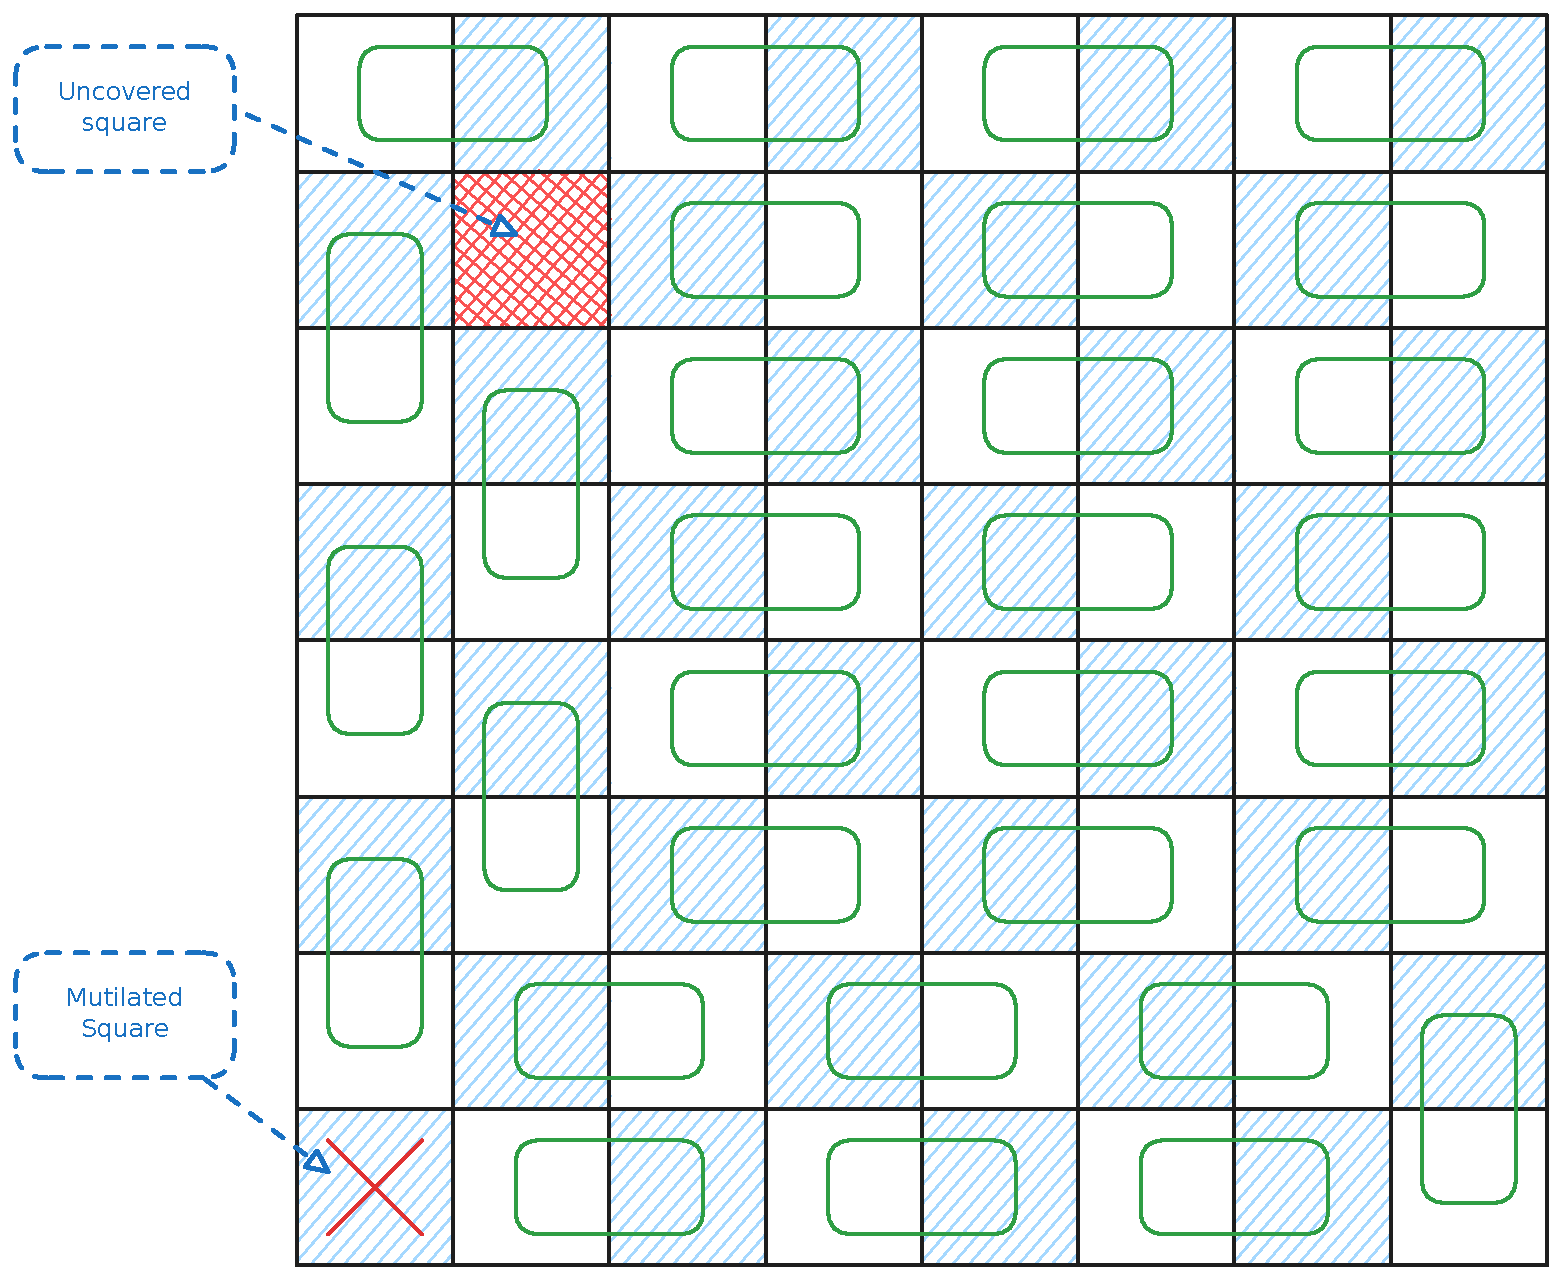
\includegraphics[width=0.7\textwidth]{Chapter2/1-mc-example.pdf}
    \caption{Example on an $8 \times 8$ chessboard with a missing square. As we can observe, there will always be one square we cannot tile }
    \label{fig:chap-2:1-mc-example}
\end{figure}



% \paragraph{Other PPAD problemsq}

% We will define several problems in \textsc{PPAD} that are related with our project
% and demonstrate the counting complexity of \textsc{PureCircuit}.

% \begin{definitionbox}{\scn{SourceOrExcess} problem \cite{ikenmeyer_WhatWhatNot_2022}}{source-or-excess}
% 	We define as $\textsc{SourceOrExcess(k,1)}$ for $k \in \mathbb{N}_{\geq 2}$
% 	the search problem as such: Given a poly-sized successor circuit $S : \mathbb{B}^n \to \mathbb{B}^n$
% 	and a set of predecessor poly-sized circuits $\{P_i\}_{i \in [k]}$, where $P_i : \mathbb{B}^n \to \mathbb{B}^n$, we define
% 	the graph $G = (V,E)$ such that, $V = \mathbb{B}^n$ and $E$ as:
% 	$$
% 		\forall x, y \in V: (x,y) \in E \iff (S(x) = y) \wedge \bigvee_{i \in [k]} P_i(y) = x
% 	$$
% 	We ensure that $0^n$ is as sink, meaning $\text{deg}(0^n) = (0,1)$.
% 	A valid solution is a vertex $v$ such that $\textit{in-deg}(v) \neq \textit{out-deg}(v)$
% \end{definitionbox}

% The $\textsc{SourceOrExcess(k,1)}$ problem can be considered as the generalisation of the \textsc{EndOfLine}
% problem for graphs with $\textit{in-deg}(\cdot) \leq k$ and $\textit{out-deg}(\cdot) \leq 1$.
% We will also introduce a planar embedding of $\scn{EndOfLine}$ on 2D grids as introduced
% by Chen et al. \cite{chen_Complexity2DDiscrete_2009}.


Lastly, we will introduce \textsc{Tarski} \ref{def:tarski-ppad}
which uses the Knaster-Tarski fixed point theorem \ref{thm:knaster-tarski} and
belongs in $\textsc{PLS} \cap \textsc{PPAD}$,
where  $\textsc{PLS}$ is a class of problems based on the idea of local search \cite{johnson_HowEasyLocal_1988}.
%
%
\begin{definitionbox}{Monotone functions}{mono-func}
    Given two partially ordered sets $(L_1, \preceq_{L_1})$ and $(L_2, \preceq_{L_2})$, a function
    $f: L_1 \to L_2$ is \textbf{monotone} if and only if:
    $$
        \forall x,y \in L_1: x \preceq_{L_1} y \implies f(x) \preceq_{L_2} f(y)
    $$
\end{definitionbox}
%     
%
\begin{theorembox}{Knaster Tarski Fixed point theorem\cite{bronislaw_TheoremeFunctionsDensembles_1928, fearnley_FasterAlgorithmFinding_2022}}{knaster-tarski}
    Given a \textit{monotone} function $f: L \to L$ \ref{def:mono-func} of a complete lattice $(L, \wedge, \vee)$,  $\exists c \in L: f(c) = c$.
\end{theorembox}

\begin{definitionbox}{$\scn{Tarski}$ problem definition \cite{fearnley_FasterAlgorithmFinding_2022}}{tarski-ppad}
    Given a \textit{monotone} function $f: L \to L$ \ref{def:mono-func} of a lattice $(L, \wedge, \vee)$
    we define solutions to the problem as:
    \begin{enumerate}
        \item Find $x \in L: f(x) = x$
        \item Find $x,y \in L$ such that $x \preceq y$ and $f(x) \not\preceq f(y)$
    \end{enumerate}
    We assume that $f$ is represented by boolean circuits.
\end{definitionbox}
%
\paragraph{Counting complexity of PPAD}
\label{par:count-ppad}


Ikenmeyer et al. \cite{ikenmeyer_WhatWhatNot_2022} demonstrated that several \textsc{PPAD-complete}
problems behave differently under $\textsc{\#PPAD} -1$. More specifically
$\textsc{\#EndOfLine} - 1 \subseteq \textsc{\#P}$ but $\exists A: \textsc{\#SourceOrExcess}^A  - 1\not\subseteq \textsc{\#P}^A$.
We estimate the counting difficulty of the aforementioned problems based on their position in the hierarchy as seen in the figure \ref{fig:ppad-count-hier}.

% \begin{figure}[h!]
%     \centering
%     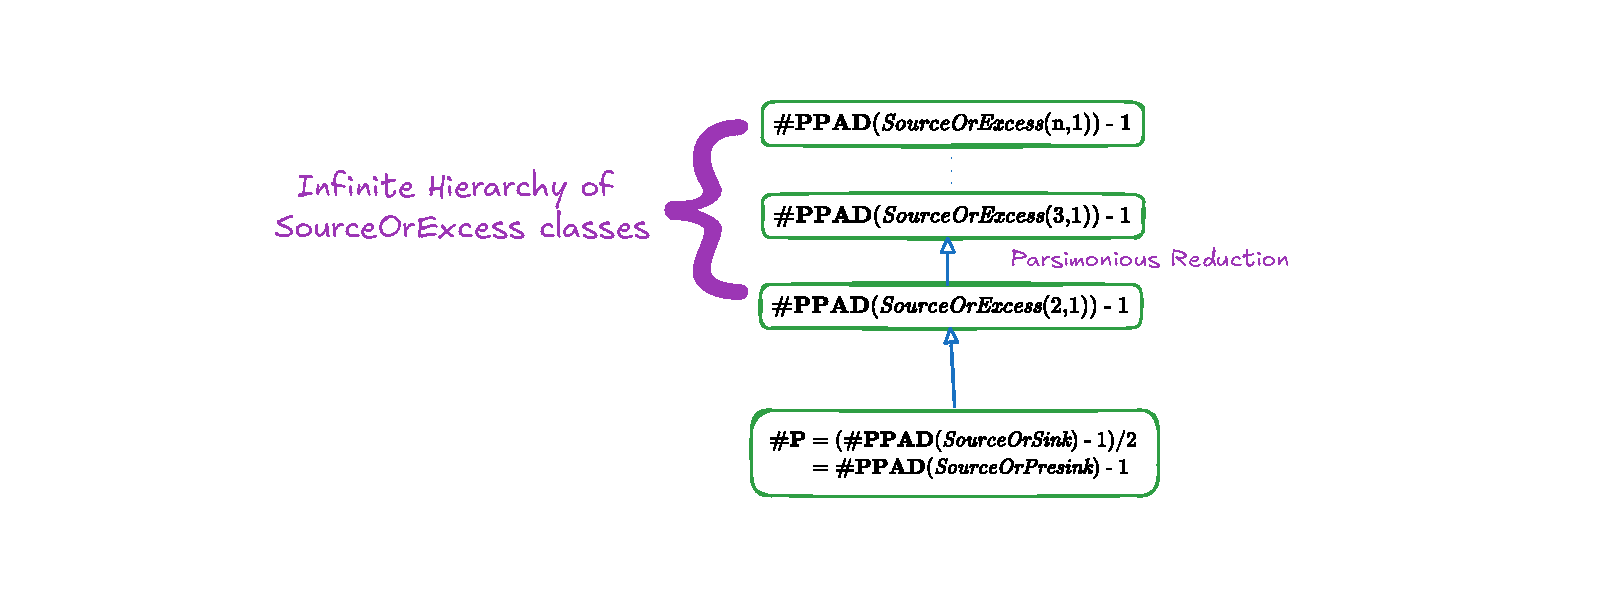
\includegraphics[width=0.75\textwidth]{assets/chart-plot.pdf}
%     \caption{Counting hierarchy graph between \textsc{\#PPAD-complete} problems. Figure obtained from \cite{ikenmeyer_WhatWhatNot_2022}.}\label{fig:ppad-count-hier}
% \end{figure}



\subsection{Counting Complexity and Combinatorial Interpretations}

Decision problems are problems that ask whether an input problem has a solution.
Search problems as we observed earlier ask what is a valid solution given the current input instance like
what is a valid colouring of a graph, satisfying assignment to a 3-SAT problem etc. Counting complexity,
or counting problems take it a step further and usually ask how many valid solutions does a problem have.
Valiant formalised this idea with the help of $\textbf{\#P}$ complexity class \ref{def:sharpp-class}, in which
he demonstrated that even if a problem is polynomially solvable in its decision/search variant, can be
much harder. A much simpler example can be found in the book by Barak et al. \cite{arora_ComputationalComplexityModern_2009}
where they provide a reduction from $\textsc{Ham-Cycle}$ to $\textsc{\#Cycle}$.


\begin{definitionbox}{\(\scn{\#P}\) Complexity Class \cite{valiant_ComplexityComputingPermanent_1979}}{sharpp-class}
    \label{def:sharpp-class}
    A function \(f: \mathbb{B}^* \to \mathbb{N} \in \textsc{\#P}\), if there exists a
    poly-function \(p : \mathbb{N} \to \mathbb{N}\) and a poly-time TM \(M\) such that:
    \[
        f(w) = \Big|\Big\{v \in \mathbb{B}^{p(|w|)} \mid M(w, v) =1 \Big\}\Big|
    \]
    Alternative but equivalent definition is as follows: A function $f \in \textbf{\#P}$,
    if there exists a non-deterministic poly-time TM $N$ such that:
    $$
        f(w) = \textbf{\#acc}_N(w)
    $$
    Where $\textbf{\#acc}_N(w)$ denotes the number of accepting paths of $N$ on $w$.
\end{definitionbox}

In hindsight, we can observe that functions in $\textbf{\#P}$ express functions of the form
$\forall w \in \{0,1\}^*: f(w) = |A_w|$, where $A_w$ is a set of objects of size
polynomial to the input.
Given the above definition, Pak et al. \cite{pak_WhatCombinatorialInterpretation_2022, ikenmeyer_PositivitySymmetricGroup_2024}
used $\textbf{\#P}$ to decide whether a class of numbers or objects have or do not have a combinatorial interpretation.
Moreover, they argue that the usage of $\textsc{\#P}$ has several benefits:

\begin{enumerate}%% TODO
    \item By polynomially bounding objects, we avoid cases such as: $f(w) = |\{1, \hdots, f(w)\}|$. In other words, we create a set
          of combinatorial objects.
    \item We can work with $f(\cdot)$, even if its direct computation is hard.
    \item $\textsc{\#P}$ is a formal system that is highly flexible.
\end{enumerate}

% The current framework was used in several papers such as
% \cite{ikenmeyer_WhatWhatNot_2022} and \cite{ikenmeyer_PositivitySymmetricGroup_2024}
% to demonstrate the existence of combinatorial interpretations.
Lastly, we introduce the idea of correlating two counting problems with the help of
\textit{parsimonious reductions}. Simply, we say
that a problem $A$ can be parsimoniously reduced to a problem $B$, if for inputs of $A$,
one can create instances of $B$ such that the set of solutions between the two problems
have the same cardinality. More formally we refer to the defintion \ref{def:pars-reduction}.
An example of how such reduction may look like, can be seen in figure \ref{fig:chap-2:pars-reduction}.


\begin{definitionbox}{Parsimonious reductions}{pars-reduction}
    Let $R, R'$ be search problems, and let $f$ be a reduction of
    $S_R = \{x \mid R(x) \neq \emptyset \}$ to $S_{R'} = \{x \mid R'(x) \neq \emptyset \}$.
    We say $f$ is \textbf{parsimonious} if:
    $$
        \forall x \in S_R : |R(x)| = |R'(f(x))|
    $$
    Where for relation $R$ we say $R(x) \triangleq \{y \in \{0,1\}^* \mid xRy \}$
\end{definitionbox}

\begin{figure}
    \centering
    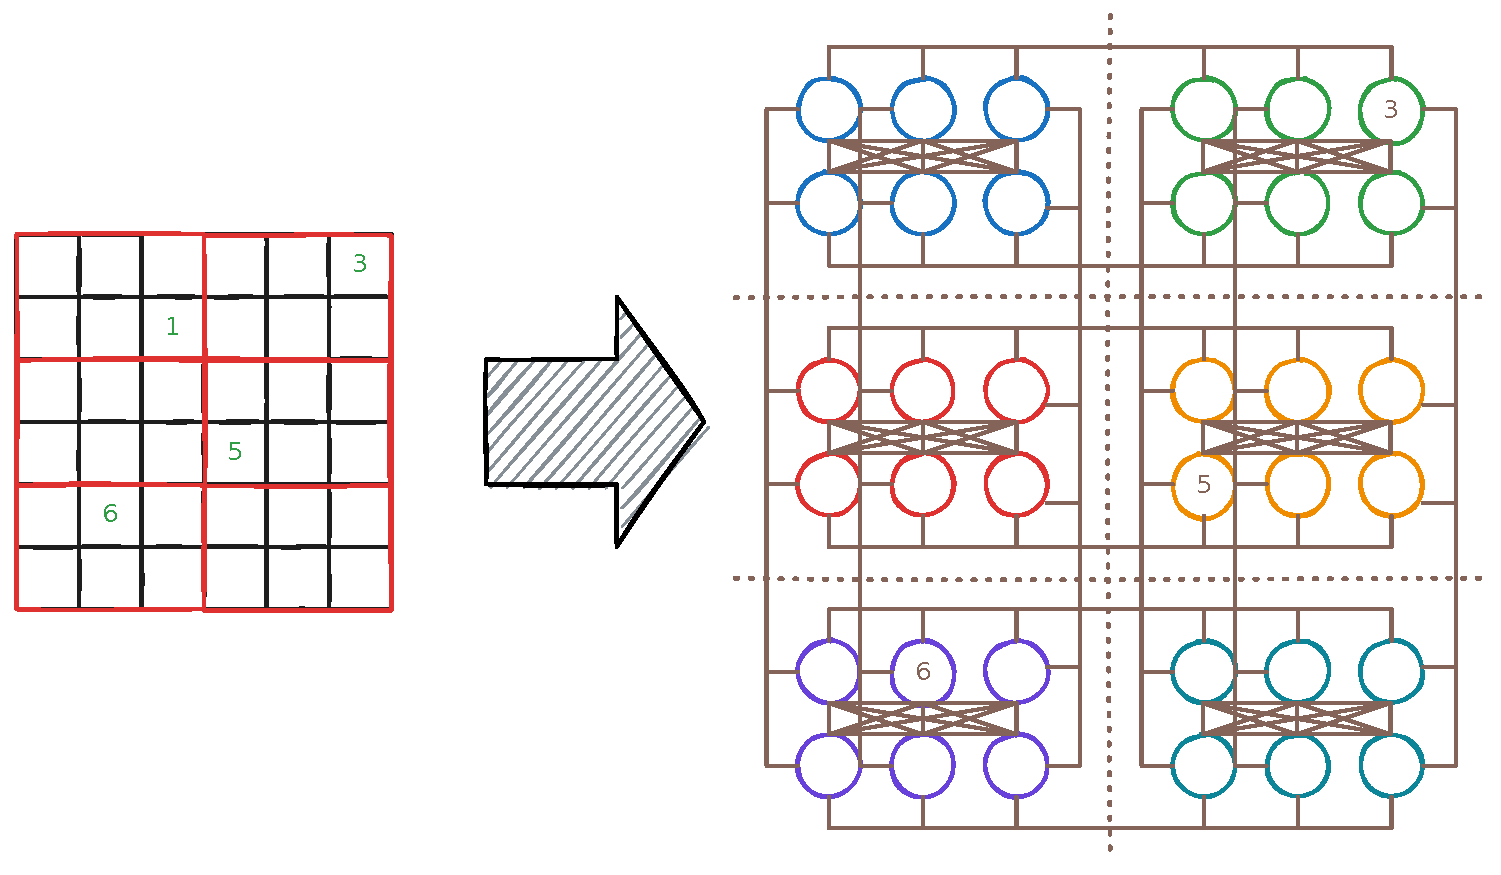
\includegraphics[width=0.5\textwidth]{Chapter2/parsimonious-reduction-example.pdf}
    \caption{Example of reducing a 6x6 sudoku puzzle, into a graph colouring problem}
    \label{fig:chap-2:pars-reduction}
\end{figure}

We introduce a more relaxed variant of parsimonious reductions in \ref{def:func-pars}
for one-to-many reductions, such that the two solutions sets are bounded by some
polynomial with respect to the size of the input. We observed that for several problems,
it can be difficult to obs

\begin{definitionbox}{Poly-Function Bounded Parsimonious Reductions}{func-pars}
    \label{def:func-pars}
    Given two counting problems $A, B : \mathbb{B}^* \to \mathbb{N}$
    and a poly-function $f : \mathbb{N} \to \mathbb{N}$, we
    say that:
    $$
        A \subseteq^f B \iff \forall x \in \mathbb{B}^n:  A(x) \leq B(x) \leq f(|x|) \cdot A(x)
    $$
    If $\forall x : f(x) = c$ for $c \in \mathbb{N}$, we use the abbreviation:
    $$
        A \subseteq^c B
    $$
\end{definitionbox}


\subsection{Kleene Logic and Hazard-Free Circuits}

Kleene logic uses the boolean system with an additional \textit{unstable} value \cite{kleene_IntroductionMetamathematics_2009}.
The study of Kleene logic assisted in
the development of robust physical systems \cite{friedrichs_MetastabilityContainingCircuits_2018} and
aiding in the development of lower bounds for monotone circuits
\cite{eichelberger_HazardDetectionCombinational_1965, ikenmeyer_ComplexityHazardfreeCircuits_2019,ikenmeyer_KarchmerWigdersonGamesHazardfree_2022,  bund_SmallHazardFreeTransducers_2025}.
The current section offers a brief summary to relevant notions and concepts in Kleene logic.

\begin{definitionbox}{Kleene value ordering \cite{mukaidono_BternaryLogicFunction_1972}}{kleene-order}
    The instability ordering for $\leq^u$ is defined as: $\bot \leq^u 0,1$. The $n$-dimensional
    extension of the ordering is:
    $$
        \forall x,y \in \mathbb{T}^n: x \leq^u y \implies \forall j \in [n]: (x_j \in \mathbb{B} \implies x_i = y_i)
    $$
\end{definitionbox}


\begin{definitionbox}{Kleene Resolutions \cite{mukaidono_BternaryLogicFunction_1972, ikenmeyer_ComplexityHazardfreeCircuits_2019}}{kleene-res}
    Given $x \in \mathbb{T}^n$, we define the \textit{resolutions} of $x$, using the following notation:
    $$
        \scn{Res}(x) \triangleq \big\{ y \in \mathbb{B}^n \mid x \leq^u y  \big\}
    $$
\end{definitionbox}

Unless otherwise specified, we assume that all Kleene functions are \textit{natural} \ref{def:nat-func}, since
they can be represented by circuits \ref{prop:nat-func-circ}.
Detecting hazards is a concept that is analysed heavily when talking about Kleene logic.
The idea is ensuring robustness in our circuits, meaning if all resolutions of $x \in \mathbb{T}^n$
give the same value, then we should expect the circuit to behave the same way \ref{def:hf-def}.
An example of hazard values can be seen in the figure \ref{fig:hazard-example}. %% TODO


\begin{definitionbox}{Natural functions \cite{ikenmeyer_ComplexityHazardfreeCircuits_2019}}{nat-func}
    A function $F: \mathbb{T}^n \to \mathbb{T}^m$ for some $n, m \in \mathbb{N}$ is \textit{natural} if and only
    if it satisfies the following properties:
    \begin{enumerate}
        \item \textit{Preserves stable values}: $\forall x \in \mathbb{B}^n: F(x) \in \mathbb{B}^m$
        \item \textit{Preserves monotonicity} \ref{def:mono-func} \ref{def:kleene-res}
    \end{enumerate}
\end{definitionbox}

\begin{propositionbox}{Natural functions and Circuits \cite{mukaidono_BternaryLogicFunction_1972,ikenmeyer_ComplexityHazardfreeCircuits_2019}}{nat-func-circ}
    A function $F: \mathbb{T}^n \to \mathbb{T}^m$ can be computed by a circuit \textit{iff} $F$ is \textit{natural} \ref{def:nat-func}
\end{propositionbox}

\begin{definitionbox}{Hazard \cite{ikenmeyer_ComplexityHazardfreeCircuits_2019, eichelberger_HazardDetectionCombinational_1965}}{hf-def}
    A \textit{circuit} $C$, on $n$ inputs has \textbf{hazard} at $x \in \mathbb{T}^n \iff C(x) = \bot$
    and $\exists b \in \mathbb{B}, \forall r \in \scn{Res}(x): C(r) = b$. If such value does not exists
    then we say that $C$ is hazard-free.
\end{definitionbox}


\begin{definitionbox}{K-bit Hazard \cite{ikenmeyer_ComplexityHazardfreeCircuits_2019}}{k-bit-haz}
    For $k \in \mathbb{N}$ a circuit $C: \mathbb{T}^n \to \mathbb{T}$ has a \textit{k-bit hazard} at $x \in \mathbb{T}^n$
    $\iff$ $C$ has a hazard at $x$ and $\bot$ appears at most $k$ times.
\end{definitionbox}

We also wish to introduce the following corollary by
Ikenmeyer et al. \cite{ikenmeyer_ComplexityHazardfreeCircuits_2019} which allows us
to construct $k$-bit hazard free circuits

\begin{corollarybox}{K-bit Hazard Construction \cite{ikenmeyer_ComplexityHazardfreeCircuits_2019}}{k-bit-haz}
    Given circuit $C: \mathbb{T}^n \to \mathbb{T}$, one can construct a $k$-bit hazard free circuit of $C$ denoted as $C'$
    such that:
    \begin{align*}
        \text{size}(C')\, & = (\frac{ne}{k})^k (\text{size}(C) + a6) + O(n^{2.71k}) \\
        \text{depth}(C') & = \text{depth}(C) + 8k + O(k \log n)
    \end{align*}
    Where $\text{size}(P)$ denotes the number of gates of $P$ and $\text{depth}(P)$ denotes the longest path from
    the input bit to the output bit
\end{corollarybox}


\subsubsection{Kleene logic and Complexity Theory}
Lastly we want to introduce the notion of \textit{Alternating Turing Machines}, which are meant to represent
a generalisation of non-deterministic Turing machines.
These have been introduced by Chandra et al. and the idea is that we introduce universal and existential quantifiers
to alternate the course of computation. The informal presentation can be thought as follows:
In a non-deterministic TM, given a single state $q$ or configuration $c$, we execute
$\beta_1, ..., \beta_k$ separate processes. We say that $q$ will accept if at least one of the processes
$\{\beta_i\}_{i \in [k]}$ accepts. Alternating Turing machines introduce additional conditions where
one accepts all $\{\beta_i\}_{i \in [k]}$ to accept or in case of a negation state, if $\beta_1$ accepts, then 
$q$ rejects or vice versa. More formally, we offer the definition in \ref{def:alt-tm}.

\begin{definitionbox}{Alteranting Turing Machines(ATM) \cite{kozen_TheoryComputation_2006, chandra1981alternation}}{alt-tm}
    \label{def:alt-tm}
    An alternating TM is a seven tuple
    $$
    M = (k , Q, \Sigma, \Gamma, \delta, q_0, g)
    $$
    Where each term denotes:
    \begin{enumerate}
        \item $K$: The number of work tapes
        \item $Q$: Finite set of states
        \item $\Sigma$: \textit{Finite} input alphabet. Moreover, $\star \not\in \Sigma$ denotes the end of the input
        \item $\Gamma$: \textit{Finite} work tape alphabet. Moreover $\# \in \Gamma$ to denote blank symbol.
        \item $\delta$ transition function or next move relation which has type of:
        $$
        \delta :Q \times \Gamma^k \times (\Sigma \cup \{\star\}) \to 
        Q \times (\Gamma \smallsetminus \{\#\})^k \times \{L, R\}^{k+1}
        $$
        \item $q_0 \in Q$: Is the initial state
        \item $g : Q \to \{\vee, \wedge, \neg , \textbf{1}, \textbf{0}\}$: Where $g$ denotes the type of state
        and $\mathbf{1}, \mathbf{0}$  denote whether it is accepting or not.

    \end{enumerate}

\end{definitionbox}

The machine essentially contains a read-only input tape with endmarkers and $k$ work tapes which are
initially blank. A \textit{step} of $m$ consists of reading a symbol from the input tape,
writing a symbol to each work tape, moving the writing head in each head left or right
while transitioning into a new state.

\begin{definitionbox}{ATM configurations \cite{kozen_TheoryComputation_2006, chandra1981alternation}}{alt-conf}
    \label{def:alt-conf}
    A configuration $\mathcal{C}$ of an ATM $M$ is a element of the set $\mathcal{C}_M$
    $$
    \mathcal{C}_M \triangleq Q \times \Sigma^* \times (\Gamma \smallsetminus \{\#\})^k \times \mathbb{N}^{k+1}
    $$
    Which represent, the current state, the input, the current contents of each work tape, and the $k+1$ head positions.
\end{definitionbox}


\section{Project Motivation and Objectives}


%!TEX root =  ../Report.tex

\section{Current findings}                               
\label{sec:findings}
We will present several attempts and efforts we made across several problems and their
parsimonious reductions.

\subsection{Attempt correlating parsimoniously PureCircuit with the EndOfLine}


% !TEX root =  ../Report.tex

\section{Chapter 4}
\label{sec: Chapter 4}
\lipsum[4]
%Here are some subsections so that they will appear on the contents

\subsection{Sub Chapter}
\label{sec: sub chapter in chapter 4}
\lipsum[5]



% !TEX root =  ../Report.tex

\section{Chapter 5}
\label{sec: Chapter 5}

\lipsum[6]

% !TEX root =  ../Report.tex

\section{Chapter 6}
\label{sec: Chapter 6}

\lipsum[7]
% !TEX root =  ../Report.tex

\section{Chapter 7}
\label{Sec: Chapter 7}

\lipsum[8]


%!TEX root =  ../Report.tex

\section{Chapter 8}
\label{sec:Chapter 8}

\lipsum[9]



% !TEX root =  ../Report.tex
\section{Making a reference}
\label{sec: Reference}

\noindent In this chapter we shall do a reference to an entry in the bibliography, \texttt{bibliography.bib}. \\

What we know of the invention of the flux capacitor is that Dr. Emmett Brown thought of this when hanging a clock in the bathroom. He was standing on his porcelain sink and slipped because it was wet, the resulting hit on the head was apparently a cause to this invention \cite{example}.\\

The corresponding sketch made on this day has been attached in appendix \ref{appx: Flux Sketch}.


%Keep adding folders as to your desires

\bibliographystyle{abbrv}
\bibliography{bibliography}

\begin{appendices}
\addcontentsline{toc}{section}{Appendices}


\section{The Flux Sketch}
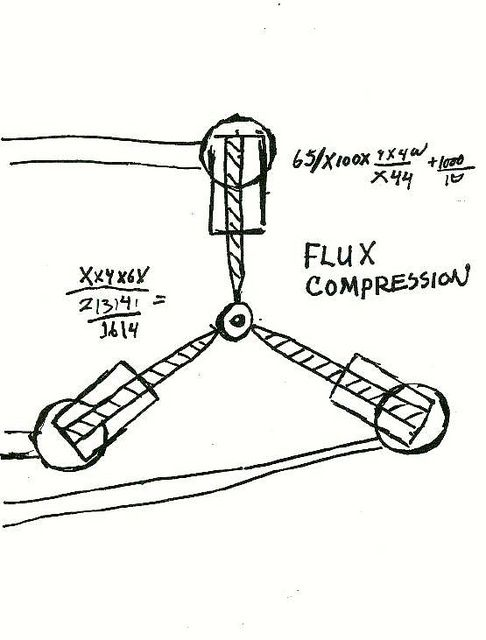
\includegraphics[width=\textwidth]{Report/Appendices/flux_sketch.jpg}
\label{appx: Flux Sketch}



\end{appendices}


\end{document}
